\documentclass[exa]{exercise_5.0}
\usepackage{hyperref}

\deadline{18.11.2024}

\begin{document}

\section{Dimensionsabhängigkeit von Zustandsdichte und Fermi-Energie}
\hfill[\href{A1}{siehe hinten }]\hspace*\fill

\section{Plasmaschwingungen in Metallen}
Mit $n(\te{Na}) = 2.53\E{22}\ufrac1{cm^3}$:
\begin{align*}
    \Aboxed{\omega_p &= \sqrt{\frac{n e^2}{\epsilon_0 m_e}} \approx 8.97 \E{15}\frac1s
    \qquad E = \hbar\omega_p \approx 5.91 \u{eV}}
\end{align*}

\section{Born-Mayer-Potential für NaCl}
\subsection{}
\begin{align*}
    U^{(C)}(r) &= -N \frac{e^2}{4\pi \epsilon_0 r}\alpha\\
    U^{(B)}(r) &= NzB \exp\hug{-\frac r\rho}\\
    U(r) &= -N \frac{e^2}{4\pi \epsilon_0 r}\alpha + NzB \exp\hug{-\frac r\rho}\\
    \\
    0&\peq \pp Ur (r_0) = N \frac{e^2}{4\pi \epsilon_0 r_0^2}\alpha - \frac{NzB}{\rho} \exp\hug{-\frac {r_0}\rho}\\
    \Aboxed{\te{\bf Gl. 1:}\quad0&= \frac{e^2 \alpha}{4\pi \epsilon_0 r_0^2}- \frac{B}{\rho}\exp\hug{-\frac {r_0}\rho}}
\end{align*}

\subsection{}
\begin{align*}
    \frac1\kappa &= V \dd[2]UV\\
    \dd[2]UV &= \dd{}V \dd UV\\
    &= \dd{}V \hug{\pp Ur \pp rV}\\
    &= \pp[2] Ur \hug{\pp rV}^2 + \underbrace{\pp Ur}_{0\te{ für }r_0} \pp[2] rV\\
    \implies \Aboxed{\dd[2]UV \eval_{r=r_0} &= \dd[2]Ur \hug{\dd rV}^2\eval_{r=r_0}}\\
\end{align*}
Mit dem Zusammenhang $V = 2 r^3 N$ gilt dann:
\begin{align*}
    \pp[2]Ur\eval_{r=r_0}&= -N \frac{e^2}{2\pi \epsilon_0 r_0^3}\alpha + \frac{NzB}{\rho^2} \exp\hug{-\frac {r_0}\rho}\\
    \dd rV &= \frac1{6 r^2 N}\\
    \\
    \dd[2]UV \eval_{r=r_0} 
    &= \dd[2]Ur \hug{\dd rV}^2\eval_{r=r_0}\\
    &= \dd[2]Ur \eval_{r=r_0} \frac1{36 r_0^4 N^2}\\
    \\
    \frac1\kappa &= \frac V{36 r_0^4 N^2} \dd[2]Ur \eval_{r=r_0}\\
    &= \frac {2 r_0^3 N }{36 r_0^4 N^2} \dd[2]Ur \eval_{r=r_0}\\
    \Aboxed{\te{\bf Gl. 2:}\quad \frac{18 r_0}{\kappa }&= - \frac{e^2}{2\pi \epsilon_0 r_0^3}\alpha + \frac{zB}{\rho^2} \exp\hug{-\frac {r_0}\rho}}
\end{align*}

\subsection{}
\inputpy{}{4.py}

Auf der Wikipedia Seite  zum \href{https://en.wikipedia.org/wiki/Buckingham_potential}{Buckingham-Potential}
ist für das Beest Kramer van Santen (BKS) Potential, einer Erweiterung des hier betrachteten Potentials, eine Liste an Parametern für häufige Materialien angegeben. Die von uns numerisch ermittelten Parameter sind in der selben Größenordnungen.

\section{Lennard-Jones-Potential}
\subsection{}
Für den Gleichgewichtsabstand muss gelten $F \propto \pp Vr =0$:
\begin{align*}
    V(r) &= 4\epsilon \bug{\hug{\frac \sigma r}^{12} - \hug{\frac \sigma r}^6}\\
    V'(r) &= 4\epsilon \bug{12\cdot \frac{-\sigma}{r^2}\hug{\frac \sigma r}^{11} - 6\cdot \frac{-\sigma }{r^2}\hug{\frac \sigma r}^5}\\
    0 &=  \hug{\frac \sigma r}^{12} - \frac12\hug{\frac \sigma r}^6\\
    \hug{\frac \sigma r}^6 &= \frac14 \pm \sqrt{\frac1{16}}= \frac 12\\
    \Aboxed{r_0 &= 2^\frac16\sigma}
\end{align*}

Die Bindungsenergie (mit positiven Vorzeichen definiert) ist dann $\abs{V(r_0)}$:
\begin{align*}
    \abs{V(r_0)} &= \abs{V(2^{\frac16} \sigma )}\\
    &= \abs{4\epsilon \bug{2^{-2} - 2^{-1}}}\\
    &= \abs{4\epsilon \bug{\frac14 -\frac12}}\\
    \Aboxed{\abs{V(r_0)} &= \epsilon}
\end{align*}

\subsection{}
Mit $m(\te{He})\approx4\u u \cdot \frac{10^{-3}}{N_A}$:
\begin{align*}
    V(r) &= 4\epsilon \bug{\hug{\frac \sigma r}^{12} - \hug{\frac \sigma r}^6}\\
    V'(r) &= -6\cdot 4\epsilon \bug{\frac 2{r}\hug{\frac \sigma r}^{12} - \frac1r\hug{\frac \sigma r}^6}\\
    V''(r) &= 24 \epsilon \sigma^6 \frac{r^6 - 2 \sigma^6}{r^{13}}\\
    \\
    V(\Delta r\ll 1) &\approx V(r_0) + \frac12\p^2 V \big |_{r_0} (\Delta r)^2\\
    \const  + \frac12 k(\Delta r)^2 &= -\epsilon + \frac12\p^2 V \big |_{r_0} (\Delta r)^2\\
    \\
    \implies k &= \p^2V\big|_{r_0} = 9\cdot 2^\frac83 \frac\epsilon{\sigma^2}= 0.792 \ufrac N{m}
\end{align*}
\begin{align*}
    c\sub{Ar} &\approx \frac12 f r_0
    = \frac{\omega r_0}{4\pi} 
    = \frac{r_0}{4\pi}\sqrt{\frac km}\\
    \Aboxed{c\sub{Ar}&\approx 331\ufrac ms}
\end{align*}
Der Literaturwert bei Raumtemperatur beträgt $c\sub{Ar} =  319 \ufrac ms $ und wurde mit einer relativen Abweichung von $3.7\%$ gut getroffen. 

\section{Fibonacci-Multilayer}
\subsection{}
In einer Fibonacci-Folge gibt es zwei Zahlen $F_0,F_1$ (meistens 0 und 1) um die Reihe zu starten, alle weiten $F_i$ ergeben sich rekursiv aus $F_i=F_{i-1}+F_{i-2}$. Übertragen auf das Schichtsystem eines Kristall ergibt sich:

\begin{table}[H]
\centering
\begin{tabular}{@{}ll@{}}
    \toprule
    $i$& $F_i$ \\
    \midrule
    0& A \\
    1& B \\
    2& AB \\
    3& BAB \\
    4& ABBAB \\
    5& BABABBAB \\
    6& ABBABBABABBAB \\
    \bottomrule
\end{tabular}
\end{table}

\subsection{}
Es gilt:
\begin{align*}
    N_{A/B}(i) &= N_{A/B}(i-1) + N_{A/B}(i-2)\\
\end{align*}
Mit den Startwerten $N_A(1) = 0, N_A(2) = 1$ und $N_B(1) = 1, N_B(1) = 1$. 
Es ergeben sich also für $N_{A/B}$ die gleichen Fibonacci-Folgen, wobei $N_B$ immer einen Schritt vorraus ist: $N_A(i) = N_B(i-1)$. 
Damit gilt für das Verhältnis $\eta = \frac{N_B}{N_A}$:
\begin{align*}
    \eta  &= \limi i\frac{N_B}{N_A} \\
    &=\limi i \frac{N_B(i)}{N_B(i-1)}\\
    &= \phi \approx \frac{1+\sqrt 5}{2}
\end{align*}

\subsection{}
Die Schichtfolge kann auch durch die Substitution 
\begin{align*}
    A \to AB \tand B \to A
\end{align*}
erzeugt werden. 

Für die Anzahl der Bausteine ergibt sich somit in Matrixdarstellung
\begin{align*}
    \binom {N_A'}{N_B'} &= \underbrace{\begin{pmatrix}
        1&1\\
        1&0
    \end{pmatrix}}_M \binom {N_A}{N_B}\begin{pmatrix}
        1
    \end{pmatrix}\\
    N(i) &= M^i N(0)\note N(i):=\binom{N_A(i)}{N_B(i)}
\end{align*}
Unter der Annahme, dass sich für $i\to \inf$ ein festes Verhältnis einstellt, heißt dies, dass der Zustandsvektor $N$ bei jeder Anwendung von $M$ maximal noch eine konstante Streckung erfahren kann. Damit ist muss $N(i\to\inf)\in \Eig{M}$, wobei der Streckungsfaktor der entsprechende Eigenwert ist.  

Die Eigenwerte sind
\begin{align*}
    0 &\peq \det(M - \lambda \I) = \begin{vmatrix}
        1-\lambda & 1\\
        1 & -\lambda
    \end{vmatrix} = \lambda(\lambda-1) - 1= \lambda^2 - \lambda -1 \\
    \lambda &= \frac12 \pm \sqrt{\frac14 + 1} = \frac{1\pm \sqrt 5 }2\\ 
    &= \phi^{\pm 1}
\end{align*}

\label{A1}
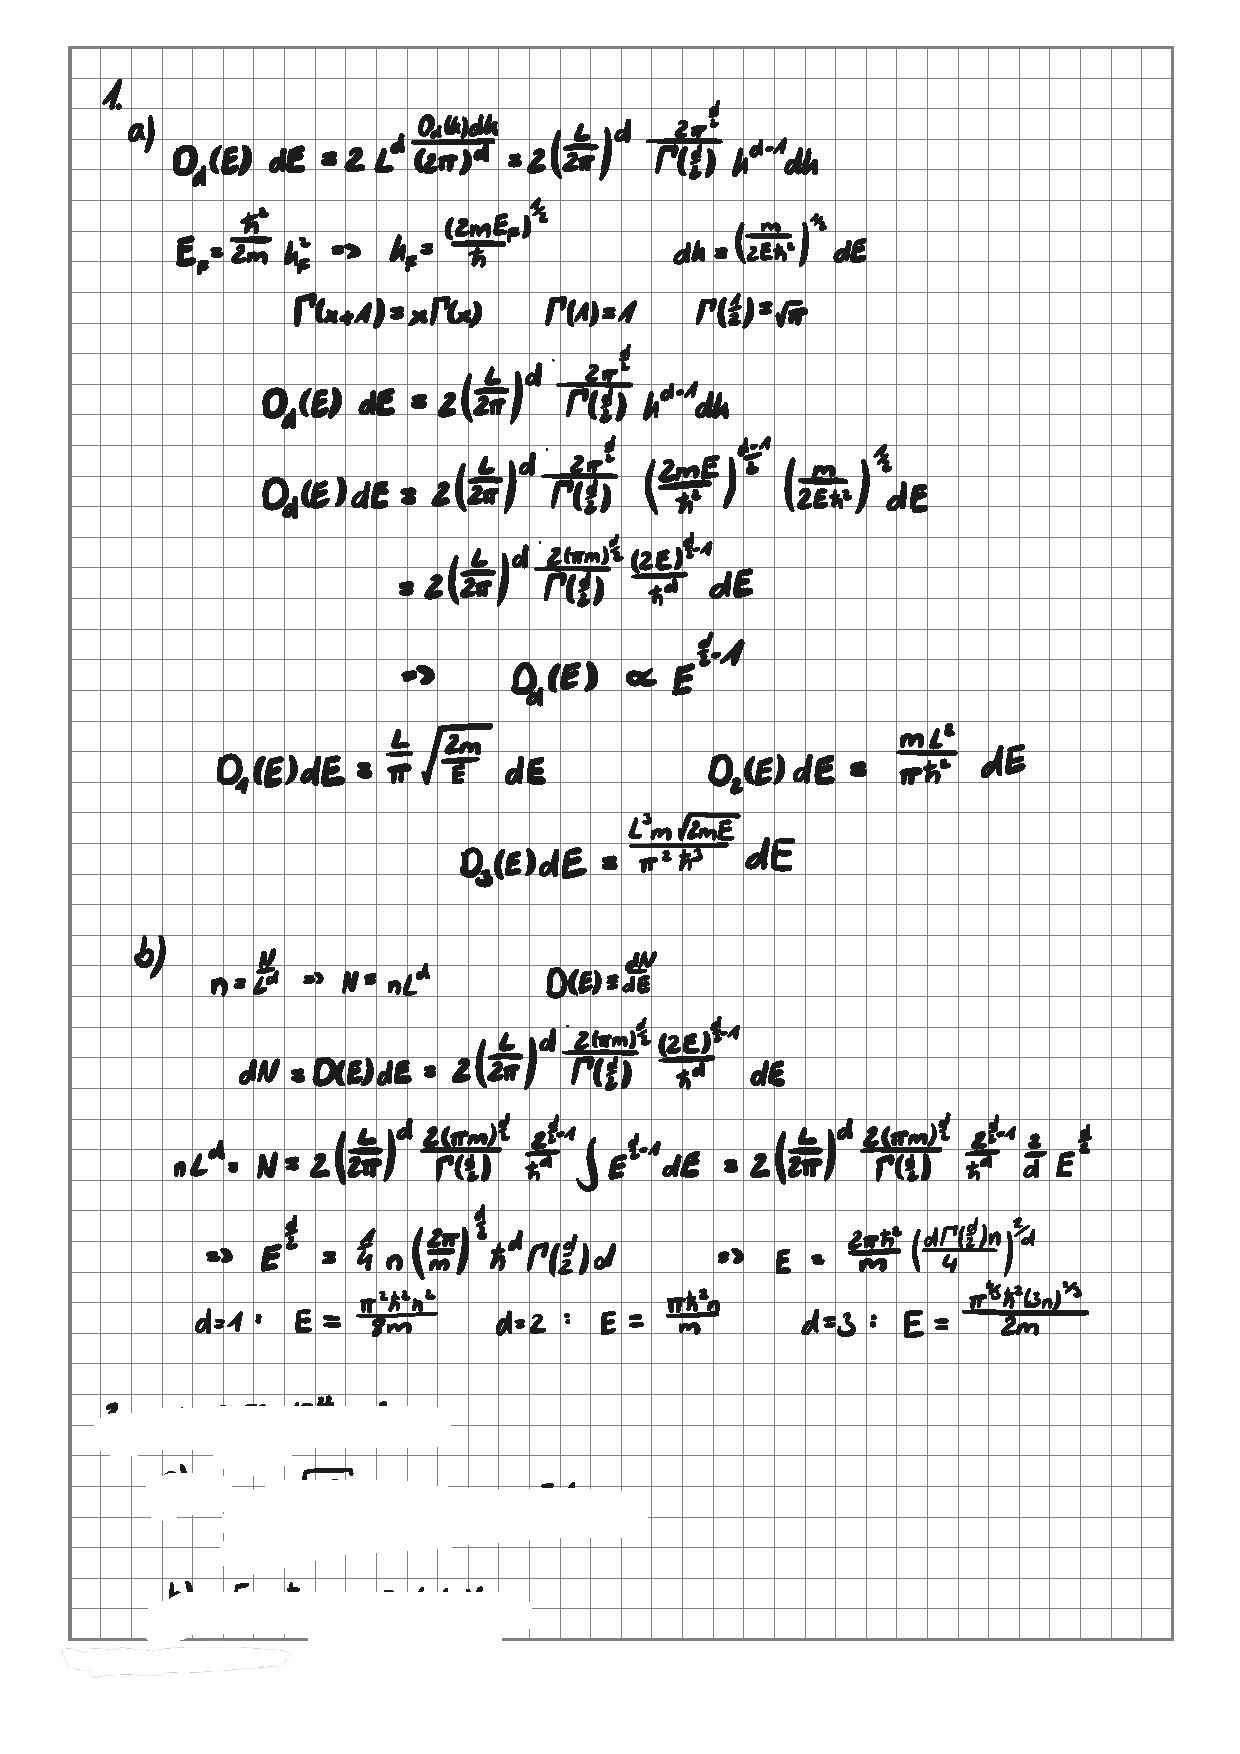
\includepdf{U4A1.pdf}

\end{document}